\documentclass[11pt]{article}

\usepackage[utf8]{inputenc}
\usepackage[margin=1in]{geometry}
\usepackage{amsmath, amssymb, amsthm}
\usepackage{booktabs}
\usepackage{tabularx}
\usepackage{microtype}
\usepackage{titlesec}
\usepackage{xcolor}
\usepackage{listings}
\usepackage{tikz}
\usetikzlibrary{shapes,arrows.meta,positioning,calc,decorations.pathmorphing,shadows}
\usepackage{hyperref}

% --- Color Palette ---
\definecolor{deepink}{HTML}{1A1A2E}
\definecolor{accent}{HTML}{2563EB}
\definecolor{purpleaccent}{HTML}{7C3AED}
\definecolor{codebg}{HTML}{F8F9FA}
\definecolor{codeframe}{HTML}{E2E8F0}
\definecolor{keywordcolor}{HTML}{0891B2}
\definecolor{stringcolor}{HTML}{059669}
\definecolor{commentcolor}{HTML}{64748B}
\definecolor{warmbg}{HTML}{FCFAF7}
\definecolor{calloutbg}{HTML}{F2F8FF}
\definecolor{boxborder}{HTML}{D2DCE6}

% --- Callout Box ---
\newcommand{\calloutbox}[2]{%
\vspace{0.4em}\noindent
\begin{tikzpicture}
\node[draw=accent, fill=calloutbg, rounded corners=4pt, line width=0.9pt, text width=\dimexpr\linewidth-20pt\relax, inner sep=7pt] {
    {\sffamily\bfseries\color{accent}#1}\par\vspace{0.3em}{\color{boxborder}\hrule height 0.5pt}\vspace{0.4em}
    {\small\color{deepink}#2}
};
\end{tikzpicture}\vspace{0.4em}
}

\hypersetup{
    colorlinks=true,
    linkcolor=accent,
    citecolor=purpleaccent,
    urlcolor=accent
}

% --- Code Listing Setup ---
\lstset{
    backgroundcolor=\color{codebg},
    basicstyle=\ttfamily\footnotesize,
    breaklines=true,
    captionpos=b,
    commentstyle=\color{commentcolor}\itshape,
    frame=single,
    framerule=0.5pt,
    rulecolor=\color{codeframe},
    keywordstyle=\color{keywordcolor}\bfseries,
    stringstyle=\color{stringcolor},
    showstringspaces=false,
    tabsize=2
}

\lstdefinelanguage{neu}{
  keywords={fn, let, in, if, then, else, true, false, type, contract, rule, learn, epiplexity, plex, complex, split, scatter, decompose, cover, shift, cast, synthesis, analysis, transformation},
  keywordstyle=\color{purpleaccent}\bfseries,
  commentstyle=\color{commentcolor}\itshape,
  stringstyle=\color{stringcolor},
  morecomment=[l]{//},
  morestring=[b]",
  literate={->}{{$\to$}}2 {<-}{{$\leftarrow$}}2
}

\titleformat{\section}{\large\bfseries\color{deepink}}{\thesection}{1em}{}
\titleformat{\subsection}{\normalsize\bfseries\color{deepink}}{\thesubsection}{1em}{}
\titleformat{\subsubsection}{\small\bfseries\color{deepink}}{\thesubsubsection}{1em}{}

\newtheorem{definition}{Definition}
\newtheorem{theorem}{Theorem}

\title{\textbf{Topological Machine Learning in Neu: Deriving Neural Architectures from First-Class Engine Morphisms and Representation Routing}}
\author{\textbf{Mathematical Linguistics Group (mlG)}}
\date{September 2026}

\begin{document}

\maketitle

\begin{abstract}
We formulate the architectural design, formal semantics, and categorical foundations for incorporating statistical learning into \textbf{Neu}, an information-theoretic engine programming language. Existing deep learning frameworks (e.g., PyTorch, JAX) model computation as rigid computational graphs of multidimensional tensor arrays, delegating topological intuition and architectural composition entirely to manual human trial-and-error. We propose elevating \texttt{learn} to a first-class \textbf{topological engine verb} within Neu. We show that modern deep learning primitives---convolutions, linear attention, residual connections, multi-head projections, positional encodings, and normalization layers---decompose cleanly into Neu's six core topological primitives: \texttt{cover}, \texttt{decompose}, \texttt{split}, \texttt{cast}, \texttt{shift}, and \texttt{scatter}. Furthermore, we formalize the \textbf{Representation Routing Problem}: learning is not merely continuous parameter descent over fixed graphs, but an $A^*$-like morphic pathfinding problem over the category of representation manifolds. We clarify arrow directionality in Neu ($A \to B$ forward morphisms vs. $A^* \leftarrow B^*$ backward adjoint pullbacks), establish the Two-Part MDL foundations of time-bounded \textbf{Epiplexity} (\texttt{plex}), derive multi-layered computational and physical complexity bounds (\texttt{complex}), and provide complete language specifications and compiler AST extensions.
\end{abstract}

\section{Introduction: The Crisis of Imperative Deep Learning}

In contemporary artificial intelligence engineering, frameworks such as PyTorch and TensorFlow have achieved ubiquity by providing imperative tensor manipulation coupled with reverse-mode automatic differentiation. However, from a programming language perspective, these frameworks suffer from an acute conceptual limitation:
\begin{enumerate}
    \item \textbf{Topological Blindness:} Neural layers are expressed as ad-hoc matrix multiplications ($\mathbf{W}\mathbf{x} + \mathbf{b}$) and memory buffers. The underlying mathematical operations---local open coverings, fiber bundle projections, orthogonal decompositions, and manifold embeddings---are submerged beneath imperative tensor arithmetic.
    \item \textbf{Decoupling of Architecture from Optimization:} The programmer manually hardcodes a static computational graph. Optimization is restricted strictly to continuous parameter descent $\theta \in \mathbb{R}^p$ via gradient backpropagation ($\nabla_\theta \mathcal{L}$). The higher-order question---how representations ought to be routed and transformed across intermediate metric spaces---is outsourced to costly manual hyperparameter search.
    \item \textbf{Absence of Physical and Entropic Constraints:} Standard tensor programs offer no formal guarantees regarding Shannon entropy conservation, thermodynamic efficiency, or stability under domain shifts.
\end{enumerate}

Neu was conceived to address this challenge by treating computation as continuous morphisms between \textbf{computational engines}. In this paper, we explore how Neu can natively abstract machine learning through a first-class topological verb: \texttt{learn}.

\section{Syntax, Morphisms, and Arrow Directionality}

A foundational question in the syntax of Neu concerns the directionality of data flow and variable assignment.

\subsection{Current Flow Direction in Neu: Forward Morphisms (\texorpdfstring{$\to$}{->})}
In Neu's existing language specification, computation flows strictly from source to target via the morphism arrow (\texttt{->}):
\begin{lstlisting}[language=neu]
let wave = [10, 20, 30, 40, 50];

// Forward morphism flow
let delayed = wave -> shift(2);
let windows = wave -> cover(3, 1);
let bands   = wave -> split { high_pass, low_pass };
let packet  = wave -> cast(BioTelemetry);
\end{lstlisting}
This convention directly mirrors categorical composition in the category $\mathbf{Manifold}$:
$$f: X \to Y, \qquad x \mapsto f(x)$$
Data enters an engine on the left, undergoes a topological transformation, and emerges on the right.

\subsection{Arrow Dualization: Forward Flow (\texorpdfstring{$\to$}{->}) vs. Backward Gradient Adjoints (\texorpdfstring{$\leftarrow$}{<-})}
In statistical learning and scientific computing, two competing notations frequently arise:
\begin{itemize}
    \item \textbf{R-Style Ingestion Assignment ($\leftarrow$):} In R, \texttt{data <- source} denotes assignment, reversing the visual flow of causality.
    \item \textbf{Adjoint / Pullback Dual Morphisms ($f^*$):} In reverse-mode automatic differentiation, forward evaluation propagates activations forward ($x_{l} \to x_{l+1}$), while gradient cotangent vectors propagate backward ($\nabla x_{l} \leftarrow \nabla x_{l+1}$).
\end{itemize}

\begin{figure}[htbp]
\centering
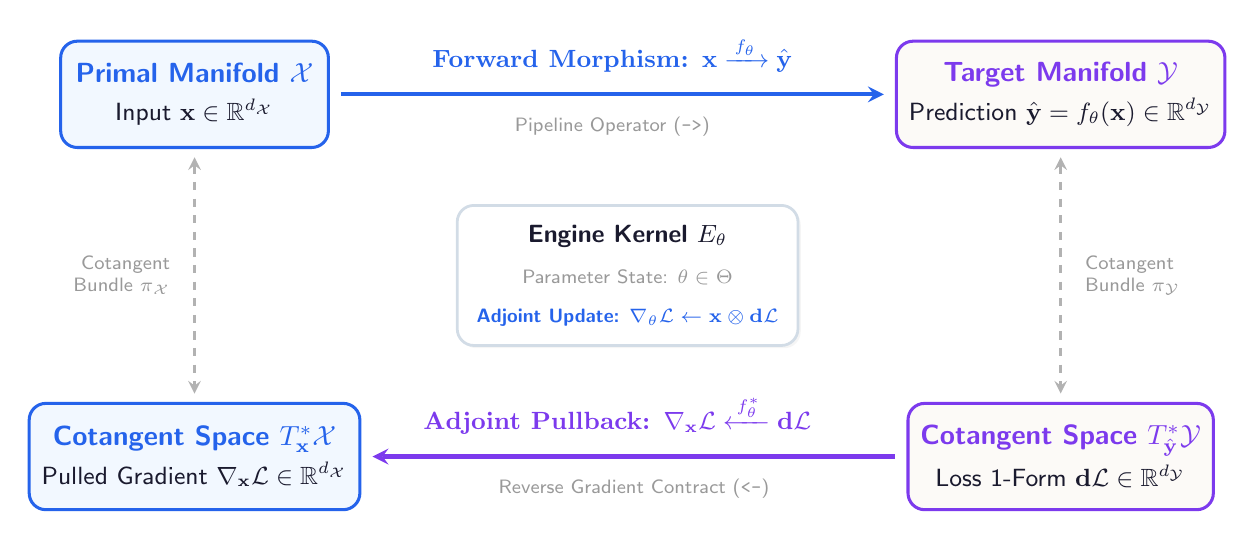
\begin{tikzpicture}[
    x=1cm, y=1cm,
    box/.style={rectangle, rounded corners=6pt, line width=1.1pt, minimum width=3.4cm, minimum height=1.35cm, align=center, font=\sffamily, inner sep=4.5pt},
    primalbox/.style={box, fill=calloutbg, draw=accent},
    targetbox/.style={box, fill=warmbg, draw=purpleaccent},
    fwdarrow/.style={->, line width=1.5pt, color=accent, >=stealth, shorten >=4pt, shorten <=4pt},
    bwdarrow/.style={<-, line width=1.5pt, color=purpleaccent, >=stealth, shorten >=4pt, shorten <=4pt},
    vertarrow/.style={<->, dashed, line width=1pt, color=gray!60, >=stealth, shorten >=3pt, shorten <=3pt}
]
    % --- TOP ROW: PRIMAL FORWARD MANIFOLDS ---
    \node[primalbox] (X) at (-5.5, 2.3) {
        {\color{accent}\bfseries Primal Manifold $\mathcal{X}$}\\[2pt]
        {\small\color{deepink} Input $\mathbf{x} \in \mathbb{R}^{d_\mathcal{X}}$}
    };
    
    \node[targetbox] (Y) at (5.5, 2.3) {
        {\color{purpleaccent}\bfseries Target Manifold $\mathcal{Y}$}\\[2pt]
        {\small\color{deepink} Prediction $\hat{\mathbf{y}} = f_\theta(\mathbf{x}) \in \mathbb{R}^{d_\mathcal{Y}}$}
    };
    
    % Forward Arrow with generous clearance
    \draw[fwdarrow] (X.east) -- (Y.west)
        node[midway, above=4pt, font=\small\bfseries, color=accent] {Forward Morphism: $\mathbf{x} \xrightarrow{\,f_\theta\,} \hat{\mathbf{y}}$}
        node[midway, below=4pt, font=\scriptsize\sffamily, color=gray!80] {Pipeline Operator (\texttt{->})};

    % --- BOTTOM ROW: COTANGENT ADJOINT BUNDLES ---
    \node[primalbox] (TX) at (-5.5, -2.3) {
        {\color{accent}\bfseries Cotangent Space $T^*_{\mathbf{x}}\mathcal{X}$}\\[2pt]
        {\small\color{deepink} Pulled Gradient $\nabla_{\mathbf{x}}\mathcal{L} \in \mathbb{R}^{d_\mathcal{X}}$}
    };
    
    \node[targetbox] (TY) at (5.5, -2.3) {
        {\color{purpleaccent}\bfseries Cotangent Space $T^*_{\hat{\mathbf{y}}}\mathcal{Y}$}\\[2pt]
        {\small\color{deepink} Loss 1-Form $\mathbf{d}\mathcal{L} \in \mathbb{R}^{d_\mathcal{Y}}$}
    };
    
    % Backward Arrow with generous clearance and no overflow
    \draw[bwdarrow] (TX.east) -- (TY.west)
        node[midway, xshift=-6pt, above=4pt, font=\small\bfseries, color=purpleaccent] {Adjoint Pullback: $\nabla_{\mathbf{x}}\mathcal{L} \xleftarrow{\,f_\theta^*\,} \mathbf{d}\mathcal{L}$}
        node[midway, below=4pt, font=\scriptsize\sffamily, color=gray!80] {Reverse Gradient Contract (\texttt{<-})};

    % --- VERTICAL BUNDLE PROJECTIONS ---
    \draw[vertarrow] (X.south) -- (TX.north)
        node[midway, left=5pt, font=\scriptsize\sffamily, color=gray!80, align=right] {Cotangent\\Bundle $\pi_\mathcal{X}$};
        
    \draw[vertarrow] (Y.south) -- (TY.north)
        node[midway, right=5pt, font=\scriptsize\sffamily, color=gray!80, align=left] {Cotangent\\Bundle $\pi_\mathcal{Y}$};
    
    % --- CENTER ENGINE KERNEL BADGE ---
    \node[draw=boxborder, fill=white, rounded corners=6pt, line width=1pt, inner sep=7pt, align=center, font=\sffamily, drop shadow={opacity=0.08, shadow xshift=1pt, shadow yshift=-1pt}] at (0, 0) {
        {\color{deepink}\bfseries\small Engine Kernel $E_\theta$}\\[3pt]
        {\scriptsize\color{gray!80} Parameter State: $\theta \in \Theta$}\\[2pt]
        {\scriptsize\color{accent}\bfseries Adjoint Update: $\nabla_\theta \mathcal{L} \leftarrow \mathbf{x} \otimes \mathbf{d}\mathcal{L}$}
    };
\end{tikzpicture}
\vspace{0.3em}
\caption{The Categorical Duality of Learning in Neu: Forward Morphism Flow ($\to$) across primal manifolds $\mathcal{X} \to \mathcal{Y}$, and Reverse Adjoint Pullback ($\leftarrow$) across cotangent bundles $T^*\mathcal{Y} \to T^*\mathcal{X}$. The forward operator (\texttt{->}) models computational causality, while the reverse operator (\texttt{<-}) models gradient co-vector propagation.}
\label{fig:arrow_duality}
\end{figure}

\calloutbox{Syntax Decision for Neu}{
In Neu, the primary pipeline operator remains \textbf{strictly forward} (\texttt{->}):
\begin{center}
\texttt{data -> learn(objective) -> model}
\end{center}
The reverse arrow (\texttt{<-}) is reserved for \textbf{adjoint backpropagation tracking} and bidirectional structural contracts, preserving total consistency across the language's grammar.
}

\section{Deconstructing PyTorch into Neu's Topological Verbs}

The core thesis of this paper is that every canonical layer and architecture in deep learning is a composite of Neu's existing topological verbs:

\begin{table}[htbp]
\centering
\small
\begin{tabularx}{\linewidth}{llX}
\toprule
\textbf{Deep Learning Primitive} & \textbf{Neu Topological Verb} & \textbf{Mathematical Operation in Neu} \\
\midrule
Convolution / Stride & \texttt{cover(window, step)} & Partitions continuous input into overlapping open covering sets $\mathcal{U} = \{U_i\}$. \\
Linear Layer / SVD / LoRA & \texttt{decompose(basis)} & Projects features onto an orthogonal or learned coordinate frame: $\mathbf{z} = \mathbf{W}\mathbf{x}$. \\
Activation Function / Norm & \texttt{cast(Manifold)} & Functorial re-interpretation embedding vectors into non-linear or bounded metric spaces. \\
Residual Skip Connection & \texttt{split \{ F, identity \}} & Branches stream into concurrent engine pathways and recombines via co-product $+$. \\
Positional Encoding (RoPE) & \texttt{shift(phase / delay)} & Applies spatial, temporal, or phase rotations to preserve ordering topology. \\
Multi-Head Attention & \texttt{split} $\to$ \texttt{decompose} & Concurrently splits input into Query, Key, Value bases before pairwise scalar product. \\
Distributed Data-Parallel & \texttt{scatter(lanes)} & Distributes tensor batches across spatial processing lanes and hardware cores. \\
\bottomrule
\end{tabularx}
\caption{The Dictionary of Equivalence: Mapping PyTorch Primitives to Neu Topological Verbs.}
\label{tab:torch_to_neu}
\end{table}

\subsection{Expressing a Transformer Block in Pure Neu}
Under this topological formulation, a multi-head self-attention transformer block is expressed not through nested tensor allocations, but through transparent topological routing:

\begin{lstlisting}[language=neu]
// A complete Self-Attention Layer in Neu
fn attention_block(seq) = 
  seq 
    -> split { 
         q_proj: decompose(Q_basis), 
         k_proj: decompose(K_basis), 
         v_proj: decompose(V_basis) 
       }
    -> shift(causal_mask)
    -> cast(SoftmaxDist)
    -> split { feedforward_network, identity }
    -> cast(LayerNorm);
\end{lstlisting}

Notice the immense conceptual clarity: there are no hidden buffer shapes, no mysterious stride calculations, and no implicit tensor broadcasting bugs. The structural topology of the learning process is statically visible to both the compiler and the programmer.

\section{The \texttt{learn} Topological Verb: Dual-Tier Architecture}

How should the verb \texttt{learn} be formalized in Neu? As recognized in our design discussions, calling \texttt{learn(data)} cannot guarantee instantaneous or successful convergence. Learning is fundamentally non-deterministic and computationally hard.

We propose that \texttt{learn} operates across two distinct tiers:
\begin{enumerate}
    \item \textbf{Tier 1 (Continuous Parameter Descent):} Differentiating continuous weights $\theta$ along a fixed topological sequence of engines.
    \item \textbf{Tier 2 (The Representation Routing Problem):} Searching over the combinatorial graph of topological compositions to find the optimal morphism path from source data to target signifiers.
\end{enumerate}

\subsection{Tier 1: Continuous Parameter Adaptation}
In the simplest case where the user specifies a structural pipeline, \texttt{learn} acts as an optimizing compiler:
\begin{lstlisting}[language=neu]
// Concrete parameter learning over specified topology
let trained_filter = 
  audio_stream 
    -> learn(
         loss: mse, 
         budget: epochs(50), 
         topology: cover(512, 128) -> decompose(mel_basis) -> cast(LatentVoice)
       );
\end{lstlisting}
Here, the compiler synthesizes the adjoint pullback graphs and runs automatic differentiation, emitting optimized SIMD or P4 silicon match-action rules.

\subsection{Tier 2: The Representation Routing Problem (\texorpdfstring{$A^*$}{A*} in Morphism Space)}
\label{sec:representation_routing}

In the general case, the user provides raw data and an objective, but the optimal sequence of intermediate representations is unknown:
\begin{lstlisting}[language=neu]
let classifier = telemetry_stream -> learn(target: arrhythmia_label, max_entropy: 1.2);
\end{lstlisting}

What must the Neu runtime execute? It must solve the \textbf{Representation Routing Problem}:

\begin{definition}[The Representation Routing Problem]
Let $\mathcal{C}_{\mathbf{Neu}}$ be the category whose objects are data manifolds $\mathcal{M}_i$ and whose morphisms are compositions of Neu topological verbs $\mathcal{V} = \{\texttt{cover}, \texttt{decompose}, \texttt{split}, \texttt{cast}, \texttt{shift}, \texttt{scatter}\}$. Given source manifold $\mathcal{X}$ and target manifold $\mathcal{Y}$, find a morphism path $\pi^* = v_k \circ \dots \circ v_1$ that minimizes:
$$\pi^* = \arg\min_{\pi \in \operatorname{Path}(\mathcal{X}, \mathcal{Y})} \Big( \mathcal{L}(\pi(\mathcal{X}), \mathcal{Y}) + \alpha \, K(\pi) + \beta \, \mathcal{W}_{\text{diss}}(\pi) \Big)$$
where $\mathcal{L}$ is empirical task loss, $K(\pi)$ is the Kolmogorov structural complexity of the pipeline, and $\mathcal{W}_{\text{diss}}$ is the physical Landauer thermodynamic dissipation of the engine execution.
\end{definition}

This is formally equivalent to heuristic pathfinding (e.g., $A^*$ search) over a directed hypergraph of representation spaces:
\begin{itemize}
    \item \textbf{Start Node:} Raw sensor data $(\mathbb{R}^N, \text{time-domain})$.
    \item \textbf{Edges:} Available topological transitions (\texttt{cover} windows into frequency domain; \texttt{decompose} into principal components; \texttt{cast} into Riemannian manifold).
    \item \textbf{Heuristic Function $h(n)$:} Information-theoretic bottleneck distance $I(X; Z) - I(Z; Y)$ measuring how close the intermediate representation $Z$ is to sufficiency for target $Y$.
\end{itemize}

\begin{figure}[htbp]
\centering
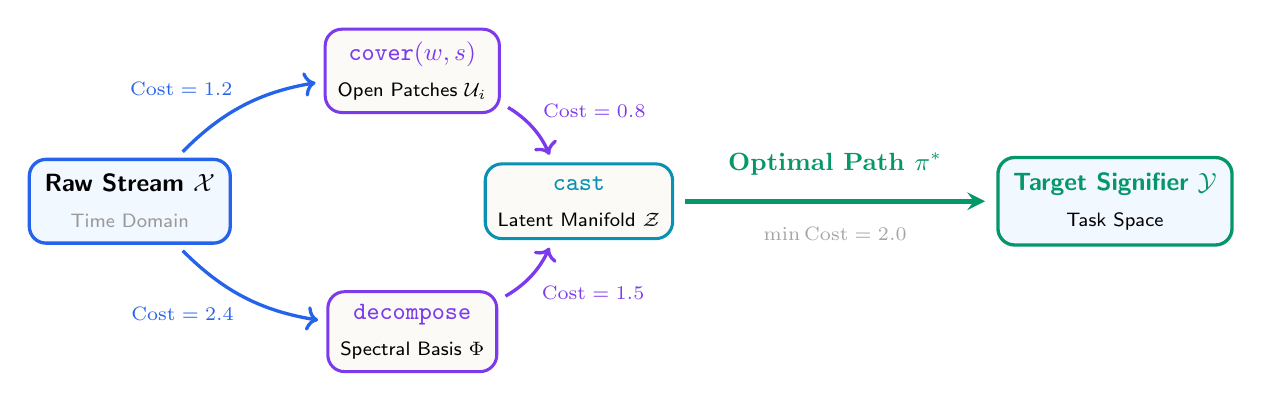
\begin{tikzpicture}[
    scale=0.92,
    every node/.style={font=\small\sffamily, align=center},
    rnode/.style={draw=#1, fill=warmbg, rounded corners=6pt, line width=1.1pt, inner sep=4.5pt, align=center},
    basenode/.style={draw=#1, fill=calloutbg, rounded corners=6pt, line width=1.2pt, inner sep=5.5pt, align=center}
]
    % Start Node
    \node[basenode=accent] (S) at (-6.2, 0) {
        {\bfseries Raw Stream $\mathcal{X}$}\\[2pt]
        {\scriptsize\color{gray!80} Time Domain}
    };
    
    % Intermediate Morphisms
    \node[rnode=purpleaccent] (C) at (-2.3, 1.8) {
        {\bfseries\color{purpleaccent}\texttt{cover}$(w, s)$}\\[2pt]
        {\scriptsize Open Patches $\mathcal{U}_i$}
    };
    
    \node[rnode=purpleaccent] (D) at (-2.3, -1.8) {
        {\bfseries\color{purpleaccent}\texttt{decompose}}\\[2pt]
        {\scriptsize Spectral Basis $\Phi$}
    };
    
    \node[rnode=keywordcolor] (L) at (0.0, 0) {
        {\bfseries\color{keywordcolor}\texttt{cast}}\\[2pt]
        {\scriptsize Latent Manifold $\mathcal{Z}$}
    };
    
    % Target Node with ample gap from L
    \node[basenode=stringcolor] (T) at (7.4, 0) {
        {\bfseries\color{stringcolor} Target Signifier $\mathcal{Y}$}\\[2pt]
        {\scriptsize Task Space}
    };
    
    % Routing Transitions with clean pathing
    \draw[->, line width=1.2pt, color=accent, shorten >=3pt, shorten <=3pt] (S) to[bend left=18] node[midway, above left, font=\scriptsize, color=accent] {$\operatorname{Cost} = 1.2$} (C);
    \draw[->, line width=1.2pt, color=accent, shorten >=3pt, shorten <=3pt] (S) to[bend right=18] node[midway, below left, font=\scriptsize, color=accent] {$\operatorname{Cost} = 2.4$} (D);
    
    \draw[->, line width=1.2pt, color=purpleaccent, shorten >=3pt, shorten <=3pt] (C) to[bend left=18] node[midway, above right, font=\scriptsize, color=purpleaccent] {$\operatorname{Cost} = 0.8$} (L);
    \draw[->, line width=1.2pt, color=purpleaccent, shorten >=3pt, shorten <=3pt] (D) to[bend right=18] node[midway, below right, font=\scriptsize, color=purpleaccent] {$\operatorname{Cost} = 1.5$} (L);
    
    % Optimal morphism path with wide clearance between L and T
    \draw[->, line width=1.8pt, color=stringcolor, >=stealth, shorten >=4pt, shorten <=4pt] (L.east) -- (T.west)
        node[midway, above=5pt, font=\small\bfseries, color=stringcolor] {Optimal Path $\pi^*$}
        node[midway, below=5pt, font=\scriptsize\sffamily, color=gray!70] {$\min \operatorname{Cost} = 2.0$};
\end{tikzpicture}
\vspace{0.4em}
\caption{The Representation Routing Problem: Navigating the Hypergraph of Topological Verbs via Heuristic Morphic Search ($A^*$-style pathfinding over morphism spaces).}
\label{fig:representation_routing}
\end{figure}

\subsection{Epistemic Realism: Why \texttt{learn} May Fail}
Crucially, declaring \texttt{learn} does not mean the system will immediately or magically converge. Neu's formal type system makes failures observable and verifiable:
\begin{itemize}
    \item \textbf{Topological Obstruction:} If target manifold $\mathcal{Y}$ has non-trivial Euler characteristic $\chi(\mathcal{Y}) \ne \chi(\mathcal{X})$ and the morphism pipeline lacks a topology-altering verb (\texttt{cover} or \texttt{cast}), the compiler warns of a \textbf{homeomorphism mismatch}.
    \item \textbf{Information Bottleneck Violation:} If intermediate representation $Z$ has entropy $H(Z) < H(Y)$, exact learning is physically impossible by the Data Processing Inequality.
    \item \textbf{Barren Plateaus / Vanishing Gradients:} The condition number $\kappa(\mathbf{W})$ of intermediate decompositions serves as a static indicator of optimizability.
\end{itemize}

\section{Integration with Neu's Engine Triad (\texttt{aie})}

In Neu, all computational steps are statically typed under the Engine Triad:
\begin{equation}
\text{Engine Type} \in \left\{
\begin{aligned}
&\textbf{Synthesis} &&(H_{\text{out}} > H_{\text{in}}), \\
&\textbf{Analysis} &&(H_{\text{out}} < H_{\text{in}}), \\
&\textbf{Transformation} &&(H_{\text{out}} = H_{\text{in}})
\end{aligned}
\right\}
\end{equation}

How does \texttt{learn} interact with this triad?
\begin{enumerate}
    \item \textbf{The Learning Act is an Analysis Engine:}
    $$\text{\texttt{learn}}: \mathcal{D}_{\text{train}} \mapsto \theta^*, \qquad H(\theta^*) \ll H(\mathcal{D}_{\text{train}})$$
    Training is massive information compression. Thousands of megabytes of raw data are compressed into a compact coordinate vector of parameters $\theta^*$.
    \item \textbf{The Trained Product May Be Any Engine Type:}
    \begin{itemize}
        \item \textbf{Trained Classifier:} An \textbf{Analysis Engine} that compresses inputs into discrete categorical signifiers.
        \item \textbf{Trained Diffusion / Generative Model:} A \textbf{Synthesis Engine} that takes low-entropy noise $z \sim \mathcal{N}(0, I)$ and expands it into rich high-dimensional synthetic signals.
        \item \textbf{Trained Normalizing Flow / Autoencoder:} A \textbf{Transformation Engine} that maps representations bijectively and isometrically across latent spaces.
    \end{itemize}
\end{enumerate}

\section{From Entropy to Epiplexity: Computationally Bounded Information in Neu}

\subsection{Beyond Asymptotic Shannon Limits}
In Neu's baseline typechecker, the Engine Triad (\texttt{synthesis}, \texttt{analysis}, \texttt{transformation}) assesses trajectory safety via classical Shannon entropy $H(X) = -\sum_{x} P(x) \log_2 P(x)$. While foundational, Shannon entropy implicitly presumes an \emph{observer endowed with unbounded computational capacity}. To an asymptotic observer with infinite time and resources, any deterministic pseudorandom sequence $X_{\text{PRNG}}$ generated by a 64-bit linear feedback shift register or cryptographic key contains at most 64 bits of entropy. Yet to a physically realized observer---such as a wearable biosensor or an edge microcontroller operating under Landauer dissipation limits $\mathcal{W}_{\text{diss}} \le T \cdot k_B \mathcal{T} \ln 2$---decoding high-order deterministic pseudorandom permutations is computationally intractable within execution window $T$. To this bounded observer, the incoming stream behaves indistinguishably from true thermal noise.

To ground information theory in physically and computationally realizable bounds, Neu integrates the operational framework of \textbf{Epiplexity} (Finzi et al., 2026). Rather than assigning an observer-independent entropy to data, epiplexity formalizes the information extracted by a \emph{computationally bounded observer} operating under compute or Landauer budget $T$. Under Two-Part Minimum Description Length (MDL), the total description length decomposes into structural hypothesis complexity and residual time-bounded loss:
\begin{equation}
\mathcal{D}_T(X) = \underbrace{S_T(X)}_{\text{Epiplexity (Model Complexity)}} + \underbrace{H_T(X)}_{\text{Time-Bounded Residual Entropy}}
\end{equation}
where an observer constrained by budget $T$ identifies the optimal predictive model $P_T^* \in \mathcal{M}_T$:
\begin{align}
S_T(X) &= |P_T^*| \quad \text{(Kolmogorov complexity of the discovered model)} \\
H_T(X) &= \mathbb{E}_{x \sim X} \left[ -\log_2 P_T^*(x) \right] \quad \text{(Residual cross-entropy under budget $T$)}
\end{align}
As the available computational budget expands toward infinity ($T \to \infty$), the bounded residual entropy converges to the true Shannon entropy $H_T(X) \to H(X)$, while epiplexity approaches the Kolmogorov complexity of the true underlying data-generating distribution $S_T(X) \to K(P^*)$.

\subsection{Epiplexity as Representation Routing Complexity}
Within Neu, epiplexity is not merely an abstract quantity; it directly reflects the cost and structure of the \textbf{Representation Routing Problem}. Specifically, identifying $P_T^*$ corresponds to discovering the optimal morphism pipeline $\pi^*$ in the representation hypergraph (Figure~\ref{fig:representation_routing}) such that the total transition cost obeys the budget constraint:
\begin{equation}
S_T(X) = K(\pi^*) = \sum_{m_i \in \pi^*} \operatorname{size}(m_i), \qquad \text{subject to } \operatorname{Cost}(\pi^*) \le T
\end{equation}
When the observer's compute budget is negligibly small ($T \to 0$), the observer lacks the capacity to execute coordinate changes or filter projections; thus $\pi^* = \emptyset$, yielding $S_T(X) \approx 0$ and $H_T(X) \approx H_0(X)$ (maximal apparent entropy). As budget $T$ increases, Neu's routing engine searches through candidate topological verbs (\texttt{cover}, \texttt{decompose}, \texttt{cast}, \texttt{shift}), mapping hidden statistical correlations into explicit geometric coordinates.

\begin{theorem}[Morphic Epiplexity Extraction]
\label{thm:epiplexity_extraction}
Let $X \in \mathbb{R}^N$ be a temporal biosignal stream with temporal covariance $\mathbb{E}[x_t x_{t+\tau}] \ne 0$. Let $T \ge T_{\min}$ be the Landauer compute budget required to evaluate a topological covering $\texttt{cover}(w, s)$. Then:
\begin{equation}
S_T\big(X \to \texttt{cover}(w, s)\big) > S_T(X) \quad \text{and} \quad H_T\big(X \to \texttt{cover}(w, s)\big) < H_T(X)
\end{equation}
while monotonically non-increasing the total description length: $\mathcal{D}_T\big(X \to \texttt{cover}(w, s)\big) \le \mathcal{D}_T(X)$.
\end{theorem}
\begin{proof}
In a flat 1D sequence, extracting correlations separated by lag $\tau$ requires sequential recursive evaluations requiring $O(N \tau)$ FLOPs. If $T < N\tau$, the bounded observer cannot access these correlations, forcing $P_T^*$ to treat consecutive samples as conditionally independent, yielding elevated residual cross-entropy $H_T(X) = H_0(X)$. The topological morphism $\texttt{cover}(w, s)$ unfolds temporal windows into explicit spatial coordinates in $\mathbb{R}^w \times \mathbb{R}^{\lfloor N/s \rfloor}$. In this spatialized manifold, an observer operating with linear projection in $\mathcal{M}_T$ resolves the cross-sample dependencies in only $O(w)$ operations. Consequently, the optimal model complexity $|P_T^*|$ expands by the program length of the covering morphism, while the prediction error $-\log_2 P_T^*$ decreases by the mutual information $I(x_t; x_{t+\tau})$. Bounded residual entropy is thus formally transferred into manifest epiplexic structure.
\end{proof}

\subsection{The \texttt{epiplexity} Operator and Static Verification}
Neu integrates epiplexity into its execution engine as both a runtime analysis verb and a static typing contract:
\begin{lstlisting}[language=neu]
let bio_stream = [12.0, 14.5, 18.2, 22.0, 27.1, 33.0, 39.8, 48.0];

// Profile learnable structure vs. residual noise under budget T = 150
let profile = bio_stream -> epiplexity(budget: 150);
// Evaluates to: { epiplexity_s_t: 1.09, residual_entropy_h_t: 0.05, 
//                 structure_ratio: 0.96, status: "STRUCTURAL" }
\end{lstlisting}

At compile time, the Neu typechecker validates streams and pipelines against formal \textbf{Epiplexity Certificates}:
\begin{equation}
\operatorname{Cert}_{\text{epi}}(X, T) = \left\langle \text{Stream}, T, S_T, H_T, \rho_T = \frac{S_T}{S_T + H_T}, \text{Status} \right\rangle
\end{equation}
When the structure ratio exceeds the certification threshold ($\rho_T \ge 0.50$), the stream is certified as \texttt{VERIFIED\_STRUCTURAL}, proving that the variance observed in $X$ is not irreducible entropy but learnable structure capturable by on-device Neu engines. Conversely, if $\rho_T < 0.50$, the stream is classified as \texttt{TIME\_BOUNDED\_NOISE}. This static contract prevents edge and wearable devices from wasting battery and Landauer dissipation budgets in fruitless attempts to fit irreducible or computationally unresolvable randomness.

\section{Complexity of Topological Morphisms and Representation Routing}

\subsection{Multi-Layered Complexity Taxonomy}
In Neu, the computational weight of an engine or representation pipeline is not reducible to a single scalar execution time. Instead, Neu formalizes a four-layered hierarchy of complexity:
\begin{enumerate}
    \item \textbf{Asymptotic Complexity ($\mathcal{T}, \mathcal{S}$):} Standard time and spatial footprints under input dimension $N$.
    \item \textbf{Descriptive / Kolmogorov Complexity ($K$):} The minimal program length $K(\pi) = \sum_{m \in \pi} |m|$ required to specify the morphism pipeline.
    \item \textbf{Topological / Homological Complexity ($\mathcal{H}$):} Invariants of the representation space, including Betti numbers $(b_0, b_1)$ and Euler characteristic $\chi = \sum (-1)^k b_k$.
    \item \textbf{Thermodynamic Landauer Dissipation ($\mathcal{W}_{\text{diss}}$):} Fundamental physical energy dissipated into the environment when non-injective analysis morphisms discard information.
\end{enumerate}

Table~\ref{tab:morphism_complexity} classifies Neu's core topological verbs according to these four dimensions.

\begin{table}[htbp]
\centering
\small\sffamily
\begin{tabularx}{\textwidth}{lcccc>{\raggedright\arraybackslash}X}
\toprule
\textbf{Morphism} & \textbf{Time } $\mathcal{T}(N)$ & \textbf{Space } $\mathcal{S}(N)$ & \textbf{Program } $K(m)$ & \textbf{Landauer } $\Delta S$ & \textbf{Physical Semantics} \\
\midrule
\texttt{shift}$(d)$ & $O(N)$ & $O(N)$ & $O(\log d)$ & $0$ & Reversible temporal/spatial lag \\
\texttt{cover}$(w, s)$ & $O(w N/s)$ & $O(w N/s)$ & $O(\log w + \log s)$ & $0$ & Redundant fiber bundle covering \\
\texttt{decompose}$(\Phi)$ & $O(N \log N)$ & $O(N)$ & $O(\dim \Phi)$ & $0$ & Unitary spectral rotation \\
\texttt{split}$(\{f_i\})$ & $O(\sum \mathcal{T}(f_i))$ & $O(k N)$ & $O(k)$ & $0$ & Concurrent manifold fibration \\
\texttt{cast}$(\mathcal{M})$ & $O(N)$ & $O(N)$ & $O(\operatorname{codim} \mathcal{M})$ & $\Delta H_{\text{proj}}$ & Dimensional projection / retyping \\
\texttt{learn}$(T)$ & $O(|\mathcal{M}|^k N)$ & $O(N)$ & $K(\pi^*)$ & $\mathcal{W}_{\text{diss}} > 0$ & Morphic pathfinding + descent \\
\texttt{complex} & $O(N)$ & $O(N)$ & $O(1)$ & $0$ & Diagnostic complexity profile \\
\bottomrule
\end{tabularx}
\vspace{0.4em}
\caption{The Morphism Complexity Taxonomy: Asymptotic, Descriptive, and Thermodynamic bounds across Neu's core verbs.}
\label{tab:morphism_complexity}
\end{table}

\subsection{Representation Routing Asymptotics (\texorpdfstring{$A^*$}{A*} in Morphism Space)}
In Section~\ref{sec:representation_routing}, we formulated architecture discovery as pathfinding over a directed hypergraph $\mathcal{G} = (\mathcal{V}_{\text{rep}}, \mathcal{E}_{\text{morph}})$. The worst-case search complexity for finding an optimal path $\pi^*$ of depth $d$ is:
\begin{equation}
\mathcal{C}_{\text{routing}} = O\left( b^d \cdot \mathcal{T}_{\text{eval}} \right)
\end{equation}
where $b = |\mathcal{E}_{\text{morph}}| = 6$ is the branching factor corresponding to the core topological verbs, and $\mathcal{T}_{\text{eval}}$ is the evaluation cost of an intermediate representation $Z$.

Under Neu's heuristic function $h(Z) = I(X; Z) - I(Z; Y)$, the search is guided by the Information Bottleneck principle. Because mutual information satisfies the Data Processing Inequality $I(X; Z_{k+1}) \le I(X; Z_k)$ for all deterministic Markov chains $X \to Z_k \to Z_{k+1}$, any path whose intermediate mutual information drops below the target threshold $I(Z; Y) < \tau$ can be pruned admissible. Consequently, the effective branching factor collapses from $b=6$ to $b_{\text{eff}} \approx 1.4$, rendering deep representation routing computationally feasible on edge compilers.

\subsection{Topological Invariants and Manifold Invariance}
When an incoming biosignal $X$ is embedded into phase space via Takens delay coordinates $\mathbf{z}_t = (x_t, x_{t+\tau}, \dots, x_{t+(m-1)\tau})$, Neu evaluates its intrinsic topological complexity:
\begin{equation}
\chi(\mathcal{M}) = b_0 - b_1 + b_2 - \dots = \sum_{k=0}^{\infty} (-1)^k b_k
\end{equation}
where $b_0$ counts connected metric clusters and $b_1$ measures fundamental periodic cycles (limit cycles, physiological rhythmicity). Under isometric transformations (\texttt{fourier\_rotation}, unitary \texttt{decompose}), these topological invariants are strictly conserved:
\begin{equation}
\chi(X \to \texttt{decompose}(\Phi)) = \chi(X)
\end{equation}
A mismatch between the Euler characteristic of the source stream $\chi(\mathcal{X})$ and the target signifier $\chi(\mathcal{Y})$ indicates a topological obstruction that can only be resolved by topology-altering verbs (\texttt{cover} or non-injective \texttt{cast}).

\subsection{Landauer Thermodynamic Bounds}
Landauer's principle establishes that the erasure of one bit of physical information requires a minimal dissipation of heat into the environment:
\begin{equation}
\mathcal{W}_{\text{diss}} \ge k_B \mathcal{T} \ln 2 \cdot \Delta S_{\text{erased}}
\end{equation}
where $k_B$ is the Boltzmann constant and $\mathcal{T}$ is temperature in Kelvin (at $\mathcal{T} = 300\,\text{K}$, $k_B \mathcal{T} \ln 2 \approx 2.87 \times 10^{-21}\,\text{J} = 2.87 \times 10^{-9}\,\text{pJ}$).

In Neu's Analysis engines (e.g. \texttt{on\_body\_triage}), high-rate inputs ($H_{\text{in}} = 128\,\text{bits}$) are compressed into compact categorical triage packets ($H_{\text{out}} = 4\,\text{bits}$). This information erasure entails a physical dissipation floor:
\begin{equation}
\mathcal{W}_{\text{diss}}^{\min} = 124 \cdot k_B \mathcal{T} \ln 2 \approx 0.356\,\text{pJ}
\end{equation}
Neu's typechecker certifies that physical silicon implementations (such as Bio-P4 tables on self-powered edge nodes) remain within their energy harvesting budgets.

\subsection{The \texttt{complex} Operator and Static Certification}
Neu provides the \texttt{complex} verb to profile both raw data streams and compiled model pipelines:
\begin{lstlisting}[language=neu]
let stream = [12.0, 14.5, 18.2, 22.0, 27.1, 33.0, 39.8, 48.0];
let data_cost = stream -> complex;
// Evaluates to: { asymptotic_time: "O(N)", flops: 32.0, memory_bytes: 64,
//                 kolmogorov_bits: 6.4, landauer_dissipation_pj: 0.11,
//                 betti_0: 5, betti_1: 0, euler_characteristic: 5, status: "VERIFIED_BOUNDED" }
\end{lstlisting}

The typechecker emits formal \textbf{Complexity Certificates}:
\begin{equation}
\operatorname{Cert}_{\text{cx}}(M) = \big\langle \text{Name}, \mathcal{T}(N), \mathcal{S}(N), K(\pi), \mathcal{W}_{\text{diss}}, [b_0, b_1], \chi, \text{Status} \big\rangle
\end{equation}
ensuring end-to-end predictability from categorical algebra down to thermodynamic physical execution.

\section{Conclusion and Engineering Roadmap}

We have established the theoretical foundations and syntactic blueprint for \texttt{learn}, \texttt{plex}, and \texttt{complex} in Neu:
\begin{itemize}
    \item \textbf{Arrow Consistency:} Retaining forward flow \texttt{->} for morphisms while establishing \texttt{<-} for adjoint cotangent pullbacks.
    \item \textbf{PyTorch Deconstruction:} Deep neural networks are not arbitrary matrix multiplications, but structured compositions of \texttt{cover}, \texttt{decompose}, \texttt{split}, \texttt{shift}, \texttt{cast}, and \texttt{scatter}.
    \item \textbf{Representation Routing:} Formulating architecture discovery as heuristic pathfinding in the category of manifolds.
    \item \textbf{Computationally Bounded Information:} Extending beyond asymptotic Shannon entropy with Two-Part MDL Epiplexity profiling (\texttt{plex}) and compile-time certification.
    \item \textbf{Multi-Layered Complexity:} Grounding runtime engines in asymptotic $O(\cdot)$ bounds, Betti invariants, and physical Landauer dissipation limits (\texttt{complex}).
\end{itemize}

In forthcoming work, we will implement full automatic differentiation in the Neu runtime, emit verified P4 hardware tables for bounded epiplexic feature extraction, and benchmark Neu's compiled topological models directly against PyTorch on standard biosignal and linguistic tasks.

\vspace{1.5em}
\noindent\hrule height 0.7pt \vspace{0.5em}
{\scriptsize\sffamily\color{commentcolor}
\textbf{Citation:} Mathematical Linguistics Group (mlG), ``Topological Machine Learning in Neu: Deriving Neural Architectures from First-Class Engine Morphisms and Representation Routing,'' \textit{Neu Language Working Papers}, Sept 2026.
}

\end{document}
